\documentclass[helvetica]{beamer}
\usetheme{Boadilla}
\input{xy}
\xyoption{all}
\usepackage{graphicx} 
\usepackage{slidesec} 
\usepackage{url}
\usepackage[framemethod=TikZ]{mdframed}
\usepackage{tikz}
\usetikzlibrary{calc,quotes,arrows.meta}
\usepackage{color}
\usepackage[normalem]{ulem}  
\setbeamertemplate{itemize items}[circle]
\def\dash---{\unskip\kern.16667em---\penalty\exhyphenpenalty\hskip.16667em\ignorespaces}
\long\def\symbolfootnote[#1]#2{\begingroup%
\def\thefootnote{\fnsymbol{footnote}}\footnote[#1]{#2}\endgroup}

\title{Privacy Preserving Measurement}
\author{Eric Rescorla \\\url{ekr@rtfm.com}}
\date{\today}

\begin{document}

\begin{frame}
  \titlepage
\end{frame}

\begin{frame}{Overview}
  \begin{itemize}
  \item Measurement scenarios
  \item Anonymous measurement
  \item MPC-based privacy-preserving measurement techniques
  \item Technical architecture
  \end{itemize}
\end{frame}

  
\begin{frame}{Many situations where we want to learn about people}

  \begin{itemize}
  \item Public research (e.g., the census)
    \begin{itemize}
    \item Demographics
    \item Income
    \item Medical issues
    \end{itemize}
    
  \item Product development
    \begin{itemize}
    \item Which features do they use/don't use?
    \item How much do they use them?
    \item Where/why are products failing?      
    \end{itemize}
    
  \item Behavioral measurements
    \begin{itemize}
    \item Discovering new Web sites
    \item Which information are people most interested in?     
    \end{itemize}
  \end{itemize}
\end{frame}

\begin{frame}{This information is very useful}

  \begin{itemize}
    \item But can be very sensitive
    \begin{itemize}
    \item Medical issues, income, sexual orientation, etc.
    \end{itemize}
  \item Even ``less'' sensitive data can be very revealing
    \begin{itemize}
    \item Especially when you put a lot of ``less'' sensitive data together      
    \end{itemize}
  \end{itemize}


  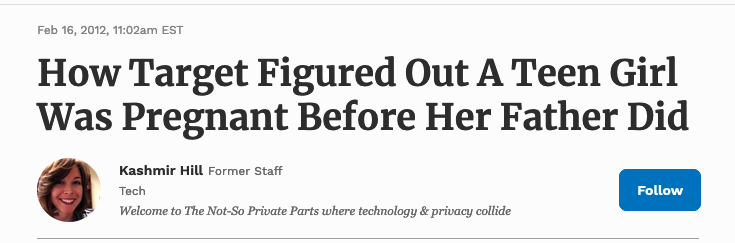
\includegraphics[scale=.3]{target-pregnancy.png}
\end{frame}


\begin{frame}{What do we really want to measure?}

  \begin{itemize}
  \item Mostly we want \emph{aggregates}
    \begin{itemize}
     \item What is the distribution of people's income?
     \item What is relationship between income and height?
     \item What are the most popular Web sites?
    \end{itemize}
  \item Need to slice the data multiple ways
    \begin{itemize}
    \item Just look at a given region
    \item Compare two variables
    \end{itemize}
  \item Individual values are neither necessary nor useful
    \begin{itemize}
    \item As long as we can compute the aggregates      
    \end{itemize}    
  \end{itemize} 
\end{frame}


\begin{frame}{Motivating Use Case: Broken Certificates}
  \begin{itemize}
  \item Firefox was seeing mysterious certificate failures in the
    field
  \item Very hard to diagnose
    \begin{itemize}
    \item We just see counts of failures      
    \item Didn't have copies of certificates or CRLs so hard to reproduce      
    \end{itemize}

  \item Much easier with a reproduction case
  \end{itemize}

\end{frame}


\begin{frame}{Motivating Use Case: Web Site Breakage}

  \begin{itemize}
  \item Web compatibility is a big problem
    \begin{itemize}
    \item Some sites will not render properly in some browsers
    \item Big problem for smaller browsers like Safari and Firefox
    \item Only a small fraction gets reported      
    \end{itemize}
    
  \item Often we can detect breakage on the client
    \begin{itemize}
    \item People hit reload or disable tracking protection
    \item API errors
    \item Call setup failures in WebRTC
    \end{itemize}

  \item No way to learn about it
    \begin{itemize}
    \item We need the URL so we can fix it
    \item But browsing history is sensitive      
    \end{itemize}

  \item Problem statement: collect the URLs with the most breakage
  \end{itemize}
\end{frame}



\begin{frame}{Preview of Other Use Cases}
  \begin{itemize}
  \item Measuring failing certificates    
  \item Advertising
    \begin{itemize}
    \item Conversion measurement
    \item Ad display measurement      
    \end{itemize}
  \item COVID Exposure notification
  \end{itemize}

\end{frame}

\begin{frame}{Measurement Types}
  \begin{itemize}
  \item Simple aggregates (mean, median, sum, histograms...)
  \item Relationships between multiple values (correlation, OLS, ...)
  \item Common strings (``heavy hitters'')    
  \end{itemize}
\end{frame}

\begin{frame}{Privacy Threats}

  \begin{itemize}
  \item Tying sensitive data directly to identifying information
    \begin{itemize}
    \item Directly via user identifiers (E-mail, cookies, etc.)
    \item Indirectly via metadata (IP address, E.164 number, etc.)
    \end{itemize}

  \item Collecting sensitive data along with non-sensitive identifying information
    \begin{itemize}
    \item Example: (birthday, zip code, initials) $\rightarrow$ income
      \end{itemize}
  \end{itemize}

  \vspace{1ex}
  \begin{quote}
    It was found that 87\% (216 million of 248 million) of the
    population in the United States had reported characteristics that
    likely made them unique based only on {5-digit ZIP, gender, date of
      birth}. --- Sweeney, 2014~\cite{sweeney2000simple}
    \end{quote}
    
\end{frame}

\begin{frame}{Anonymized Data Collection}

  \begin{itemize}
  \item Basic idea: collect user information without identifiers
  \item Practically speaking    
    \begin{itemize}
    \item Strip direct identifiers on the client side
    \item Strip metadata using a proxy
    \end{itemize}    
  \end{itemize}

  \vspace{2ex}
  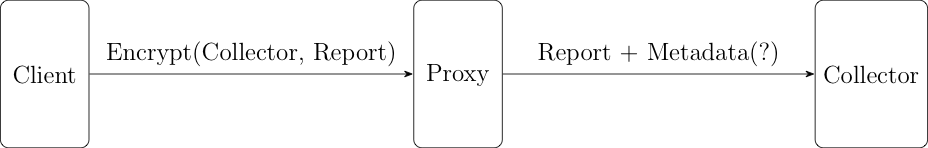
\includegraphics[width=4in]{anonymizing-proxy}
  \vspace{2ex}
  
  \begin{itemize}
  \item Example technologies:
    \begin{itemize}
    \item Connection-level proxies (IPsec, RFC 2817 CONNECT, MASQUE)
    \item Application-level proxies (OHAI)      
    \end{itemize}
  \end{itemize}
\end{frame}


\begin{frame}{Good Use Cases for Anonymization}

  \begin{itemize}
  \item Boosting the privacy of semi-sensitive data
    \begin{itemize}
    \item Example: existing browser Telemetry is done with no privacy
    \end{itemize}

  \item Individual values where you don't need to ``dig into'' the data
    
  \item Freeform data
    \begin{itemize}
    \item E.g., JSON blobs
    \end{itemize}

  \item Anything that needs an answer
    \begin{itemize}
    \item DNS requests
    \item Safe Browsing queries
    \end{itemize}
  \end{itemize}
\end{frame}


\begin{frame}{Bad Use Cases for Anonymization}

  \begin{itemize}
  \item High dimensionality data
    \begin{itemize}
    \item Multiple variables that need to be reported together
    \item When you want to look at subgroups
    \item Any time you want to do correlation/regression
    \item \emph{Anonymized data needs to be disaggregated to prevent de-anonymization}
    \end{itemize}

  \item Collecting common values
    \begin{itemize}
    \item The ``top N'' values
    \item Only values common to $>N$ users
    \item \emph{Anonymized data collects every value and depends on reporting only common values}      
    \end{itemize}
  \end{itemize}
\end{frame}


\begin{frame}{Cryptography to the Rescue}
{\center
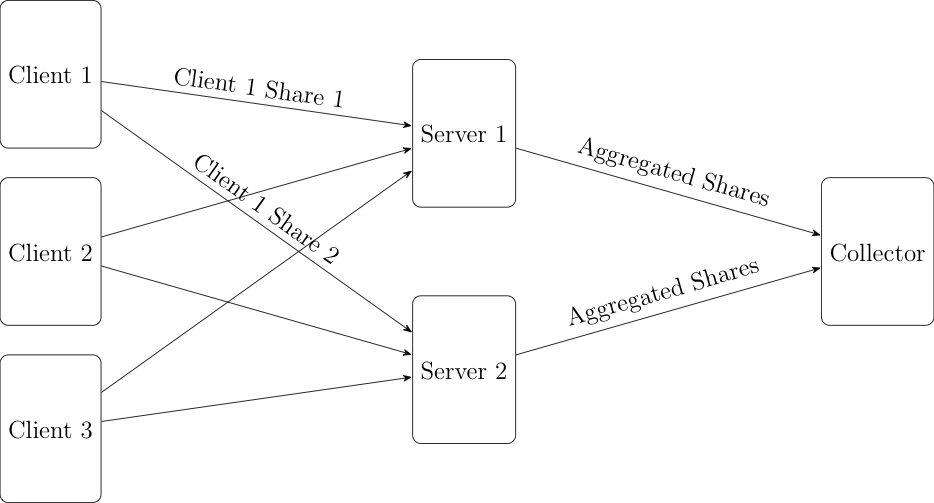
\includegraphics[width=4in]{prio.png}  
}
\begin{itemize}
\item Split data between two servers
\item Each server computes aggregated shares
\item Aggregate shares combined to produce final value  
\end{itemize}
\end{frame}

\begin{frame}{Example: Prio~\cite{201553}}

  \begin{itemize}
  \item Useful for computing numeric aggregates (sum, mean, etc.)
  \item[]
  \item Each client $i$ holds a value $x_i$
    \begin{itemize}
    \item Generates random $R_i \leftarrow \mathbb{F}_p$
    \item Sends $x_i - R_i (mod p)$ to server 1
    \item Sends $R_i$ to server 2
    \end{itemize}

  \item Each server adds up their shares
    \begin{itemize}
    \item Server 1: $\sum_i x_i - R_i$
    \item Server 2: $\sum_i R_i$
    \end{itemize}

  \item Now add these up: $\sum_i x_i - R_i + \sum_i R_i = \sum_i x_i + \sum_i R_i - \sum_i R_i = \sum_i x_i$
  \end{itemize}
\end{frame}


\begin{frame}{What else can Prio compute?}

  \begin{tabular}{l l}
    Arithmetic mean & $\sum_i x_i / i$ \\
    Product & $exp(\sum_i log(x_i))$  \\
    Geometric mean & From product \\
    Variance and stddeviation & From $\sum_i x_i$ and $\sum_i (x_i)^2$ \\
    Boolean OR, AND & ... \\
    MIN, MAX & ... \\
    Ordinarily least squares (OLS) & ... \\
  \end{tabular}

  \vspace{2ex}
  \begin{itemize}
    \item[] The trick is finding the right encoding    
    \end{itemize}
\end{frame}

\begin{frame}{What about bogus data?}

  \begin{itemize}
  \item Plausible but false
    \begin{itemize}
    \item ``I am 180cm tall'' when I am actually 175cm
    \item A problem with any surveying technique
    \item We just live with them
    \end{itemize}
  \item Completely ridiculous
    \begin{itemize}
    \item ``I am 1km tall'' (or worse, ``I am -1km tall'')
    \item Easy to remove with standard systems by filtering
      \begin{itemize}
      \item ... but with Prio the data is encrypted
      \end{itemize}

    \end{itemize}
  \item Solution: each submission comes with a zero-knowledge proof of validity
    \begin{itemize}
    \item ``This height report is between 100 and 200cm''
    \item Servers work together to validate the proof
    \item Only aggregate submissions with valid proofs
    \end{itemize}
  \end{itemize}
\end{frame}


\begin{frame}{Heavy Hitters~\cite{cryptoeprint:2021:017}}

  \begin{itemize}
  \item Each client submits a string (e.g., a URL)
    \begin{itemize}
    \item Report the $N$ most frequent strings
    \end{itemize}

  \item Servers jointly can compute the number of strings with prefix $p$
    \begin{itemize}
    \item Can use binary search to compute the most common strings
    \item ``How many strings have prefix $p || 0$ versus $p || 1$
    \end{itemize}
  \end{itemize}

 % TODO: binary tree picture?
\end{frame}



\begin{frame}{Subset Queries}

  \begin{itemize}
  \item Submissions can be tagged with demographic data
    \begin{itemize}
    \item Example: (birthday, zip code, initials) $\rightarrow$ Encrypted(income)
    \item This is safe because the sensitive information is encrypted      
    \item Servers can then compute aggregates over subsets
    \end{itemize}

  \item Repeated queries can be used to determine individual values
    \begin{itemize}
    \item Querying for $S$ and $S \setminus I$ reveals $I$'s value
    \item Defenses
      \begin{itemize}
      \item Minimum batch size
      \item Anti-replay
      \item Differential privacy randomization
      \end{itemize}
    \end{itemize}
  \end{itemize}
\end{frame}


\begin{frame}{Privacy Preserving Measurement Protocol}
  {\texttt{draft-gpew-priv-ppm-00}}

  \begin{itemize}
  \item A generic protocol for privacy-preserving measurement
    \begin{itemize}
    \item Compatible with multiple cryptographic algorithms (``verifiable distributed aggregation functions'')
    \end{itemize}

  \item Build on top of HTTPS
    \begin{itemize}
    \item Easy to implement with existing services infrastructure
    \end{itemize}
  \end{itemize}
\end{frame}

\begin{frame}{PPM System Architecture}

{\center
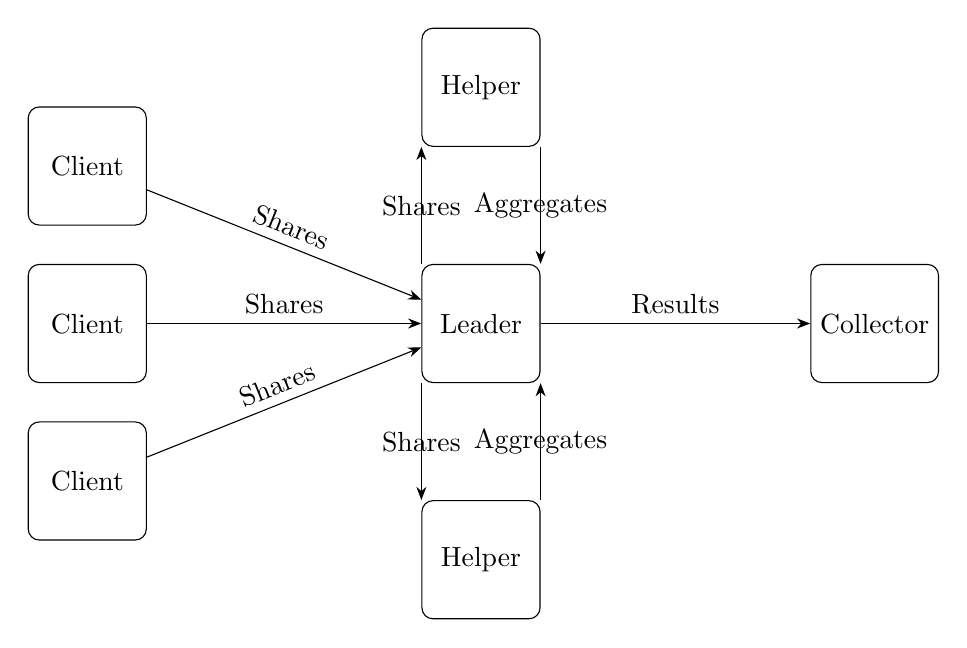
\begin{tikzpicture}
[
 device/.style={rectangle, minimum height=1.5cm, minimum width=1.5cm, draw, rounded corners, align=center},
 >=Stealth
 ]

 \node (client1) at (0, -2) [device] {Client};
 \node (client2) at (0, 0) [device] {Client};
 \node (client3) at (0, 2) [device] {Client};

 \node (helper1) at (5, -3) [device] {Helper};
 \node (leader) at (5, 0) [device] {Leader};
 \node (helper2) at (5, 3) [device] {Helper};

 \node (collector) at (10, 0) [device] {Collector};
 
 \path [->] (client1) edge node [above, sloped] {Shares} (leader);
 \path [->] (client2) edge node [above] {Shares} (leader);
 \path [->] (client3) edge node [above, sloped] {Shares} (leader);

 \path [->] (leader) edge node [above, sloped] {Results} (collector);

 \path [->] (leader.north west) edge node {Shares} (helper2.south west);
 \path [->] (helper2.south east) edge node {Aggregates} (leader.north east);

 \path [->] (leader.south west) edge node {Shares} (helper1.north west);
 \path [->] (helper1.north east) edge node {Aggregates} (leader.south east);


\end{tikzpicture}
}


\end{frame}

\begin{frame}{Questions?}

\end{frame}

\bibliography{ppm}
\bibliographystyle{alpha}

\end{document}


        